\section{Introduction}

Engineers solve problems. Regardless of field, discipline, and generation, every engineer
strives to solve problems. While the need for problem solvers does not change with time,
the methods for solving problems certainly do. Consider the process of creating detail 
drawings. Engineers needed a way to communicate the size, shape, and finish of parts to 
other engineers, so they hand drew and dimensioned parts. But in the modern day, 
hand drafting a detail drawing is the last resort. And education has adjusted in
kind. While students are taught to draw straight lines and visualize
without the aid of CAD, no class spends time teaching students how to use a drafting table
or create detail drawings by hand. Rather, they are taught the basics of visualization
and then taught how to use a CAD program, like SOLIDWORKS.

The same could be said for setting the state in a thermodynamics problem, graphing
deflection in a load-bearing beam, or finding the Q-value of a fission reaction. At one
point, looking up values in a table and plugging them into a calculator or using a ruler
and lined paper were state-of-the-art methods for solving these problems. However, as the 
times change, so do the methods, and with the advent of programming and its ever lowering 
barrier to entry, these problems can more easily, and more accurately, be solved with a 
simple script in any number of programming languages.

Despite this, most classes continue to have students spend hours thumbing through tables
to solve every problem by hand. In contrast to this, other classes have recognized the
value of modern solution methods and rely heavily on them, only to find that students
lack sufficient training to effectively utilize them. Because of this dichotomy, a cohesive 
and consistent programming ecosystem should be adopted throughout the curriculum 
of the Mechanical and Nuclear Engineering department.


\section{Background}

The first introduction to programming in MNE curriculum is DEN 161: Engineering Problem Solving,
the first-semester introduction-to-engineering class. The class spends a few weeks introducing
Python and then a week introducing the Arduino Uno. After this, no programming is formally used in the
curriculum until first semester Junior year, as seen in Figure \ref{fig:mne_flowchart}
\cite{flowchart2022}. 

\begin{figure}[!htbp]
    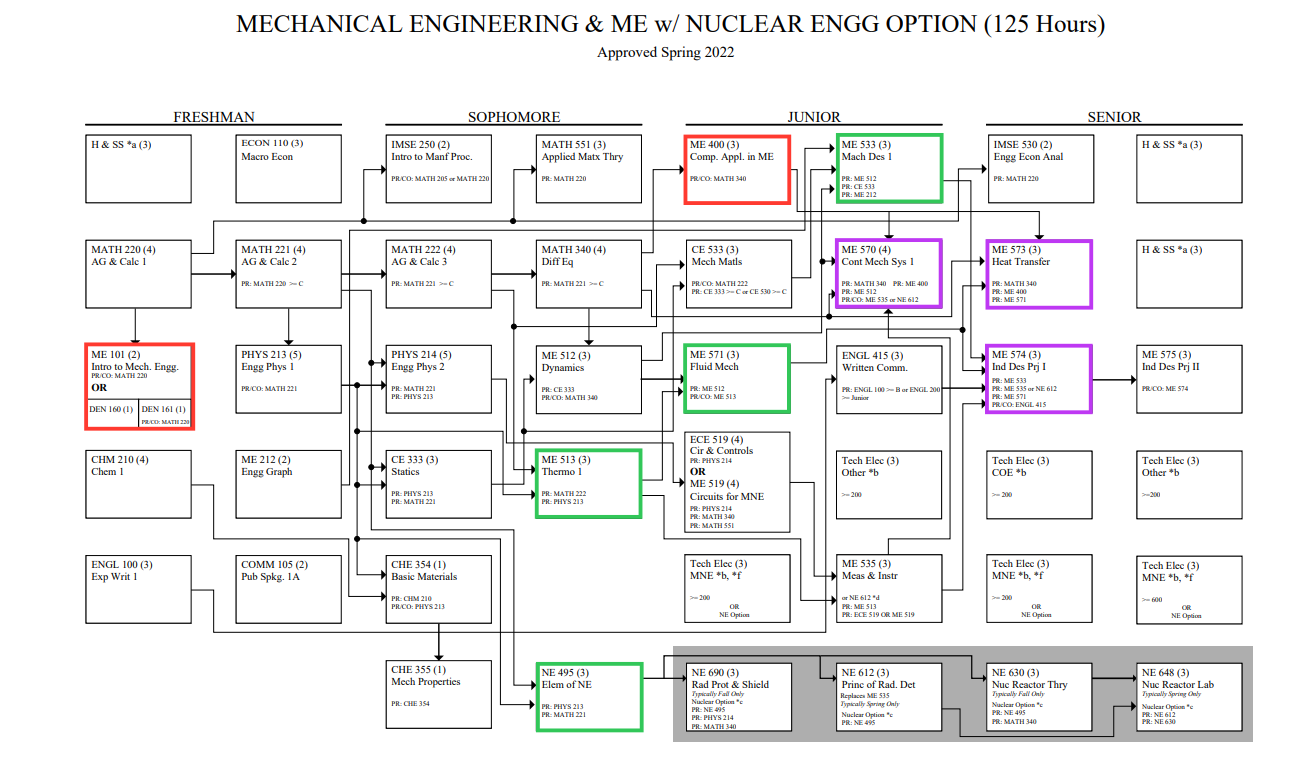
\includegraphics[angle=90, scale=0.6]{mne-flowchart}
    \begin{tabular}{l@{ : }l}
        Red & Teaches Programming \\
        Purple & Uses Programming \\
        Green & Does not utilize Programming, but could \\
    \end{tabular}
    \centering
    \caption{MNE Curriculum Flowchart}
    \centering
    \label{fig:mne_flowchart}
\end{figure}

The next class to use programming is also the only class dedicated to teaching programming.
ME 400: Computer Applications in Mechanical Engineering begins with an introduction to C++
but then quickly moves to teaching embedded C++ for use on an ESP32. While the class
contains useful material as it relates to embedded programming, students often comment on
the fast-paced nature of the course.

The next class to utilize programming is ME 570: Control of Mechanical Systems 1. This class
uses MATLAB for system analysis and controller design. For the first lab, students complete the
MATLAB Onramp, MATLAB's own introductory course to the language. This Onramp, however, does
not cover the basics of the control package that the course relies on. Due to their inadequate 
foundations in programming, many students struggle with the new language, making it difficult 
to understand the new concepts being taught, such as a PID controller.

The final class that utilizes programming is ME 574: Interdisciplinary Design Project 1, 
better known as Senior Design 1. This class revolves around the completion and fabrication
of a single product. This product is designed to always have some electromechanical aspects that need to
be controlled by a microcontroller. Neither the device nor language used is moderated by
the class instructors. Since this is a project based class where each team is responsible
for its own decisions and the project changes every semester, it will not receive a dedicated
chapter or assignment redesign.

As it currently stands, the MNE department makes use of three different programming languages
in required classes: C++, MATLAB, and Python. While each of these languages and 
environments come with advantages, and the idea of learning multiple languages has merit,
many students find themselves confused by the variety. Rather than
feeling competent in one language, they feel incompetent in three.

In addition to the unstable foundation and lack of consistency, the use of programming is 
absent from several classes that would benefit from its inclusion. Classes that spend
substantial time with property tables, iterative design, or numerical methods
showcase the power of programming in the field of mechanical engineering. 

Based on experience as an instructor of ME 570 and ME 574 for the better part of 
four years, I have found that the majority of students struggle with using MATLAB and C++. 
This makes it 
difficult for students to learn engineering principles because they do not understand 
the tool being used to teach it. But, at the same time, it is important to use modern
techniques to solve problems.

\section{Scope of Work}

While the motivation for this work is centered on the idea that a more consistent approach to
learning and applying programming would benefit students and improve their problem-solving
abilities, this project does not seek to prove or verify this claim. Neither does this
work set out to prove that the proposed solution is the best solution for the assumed
problem. This project merely seeks to identify a potential path forward while 
demonstrating both the advantages and disadvantages of the curriculum. 

This work will take time to point out benefits and drawbacks compared to the current 
curriculum, but given that no other possible solution is considered, it would be
premature to draw conclusions relating to the ``best'' path forward. However, there 
will be a brief discussion of alternative options in the concluding chapters of the paper.

\section{Structure of Work}

Since this body of work does not set out to prove a hypothesis, opting instead to demonstrate
a consistent usage and application of programming across the MNE curriculum, the format of
this paper will be adjusted accordingly. The next chapter, titled ``A Cohesive Programming
Curriculum,'' will discuss the foundation of the new implementation, such as the language,
hardware, and development environment. It will also discuss the general goal of the changes.

Subsequent chapters will each be dedicated to a class in the MNE curriculum. These chapters
will give a course overview, describe the new or altered assignments, give a list
of deliverables for that course, and provide recommendations for implementation. Complete 
assignment descriptions and implementations
are not contained within the chapters themselves; only representative portions are included.
The assignments are contained in a repository on GitHub, which can be found in Appendix 
\ref{appendix:appendix_github}. Each chapter will have a folder of the same name dedicated 
to it in the repository. This folder will contain everything an instructor would need to assign 
and grade the new assignments.

\section{Curriculum Design}

When designing assignments and their implementations, the fundamentals of curriculum design
help guide both the progression and weighting of assignments. As such, considerations were
made for the integration of programming both on a per-class and a program-wide basis.

In a 2009 study, Meyers and Nulty use five guiding principles for the alignment of learning
environments, assessment, learning approaches, and learning outcomes \cite{5-cd-principles}.
The authors state that student learning will be maximized when students are provided
with teaching, learning materials, tasks, and experiences that:
\begin{enumerate}
    \item are authentic, real-world and relevant;
    \item are constructive, sequential and interlinked;
    \item require students to use and engage with progressively higher order cognitive 
    processes;
    \item are all aligned with each other and the desired learning outcomes; and
    \item provide challenge, interest and motivation to learn. \cite{5-cd-principles}
\end{enumerate}

The programming implementation provided in this paper attempts to adhere to all five
principles. The problems given all represent real-world problems and attempt to use
modern solution methods, similar to those used in industry, to solve them. The assignments
come as a natural progression from learning the engineering principles, applying them by
hand, and then solving them with software. The curriculum also pushes the students to 
participate in ``progressively highly order cognitive processes'' through the use of 
increasingly complex assignments and expectations. These assignments use a revision of
Bloom's Taxonomy proposed by Krathwohl in 2002 to create assignments with the appropriate
difficulty \cite{revised-bloom}. This progression can be seen in Figure \ref{revised-bloom-taxonomy}.

\begin{figure}
    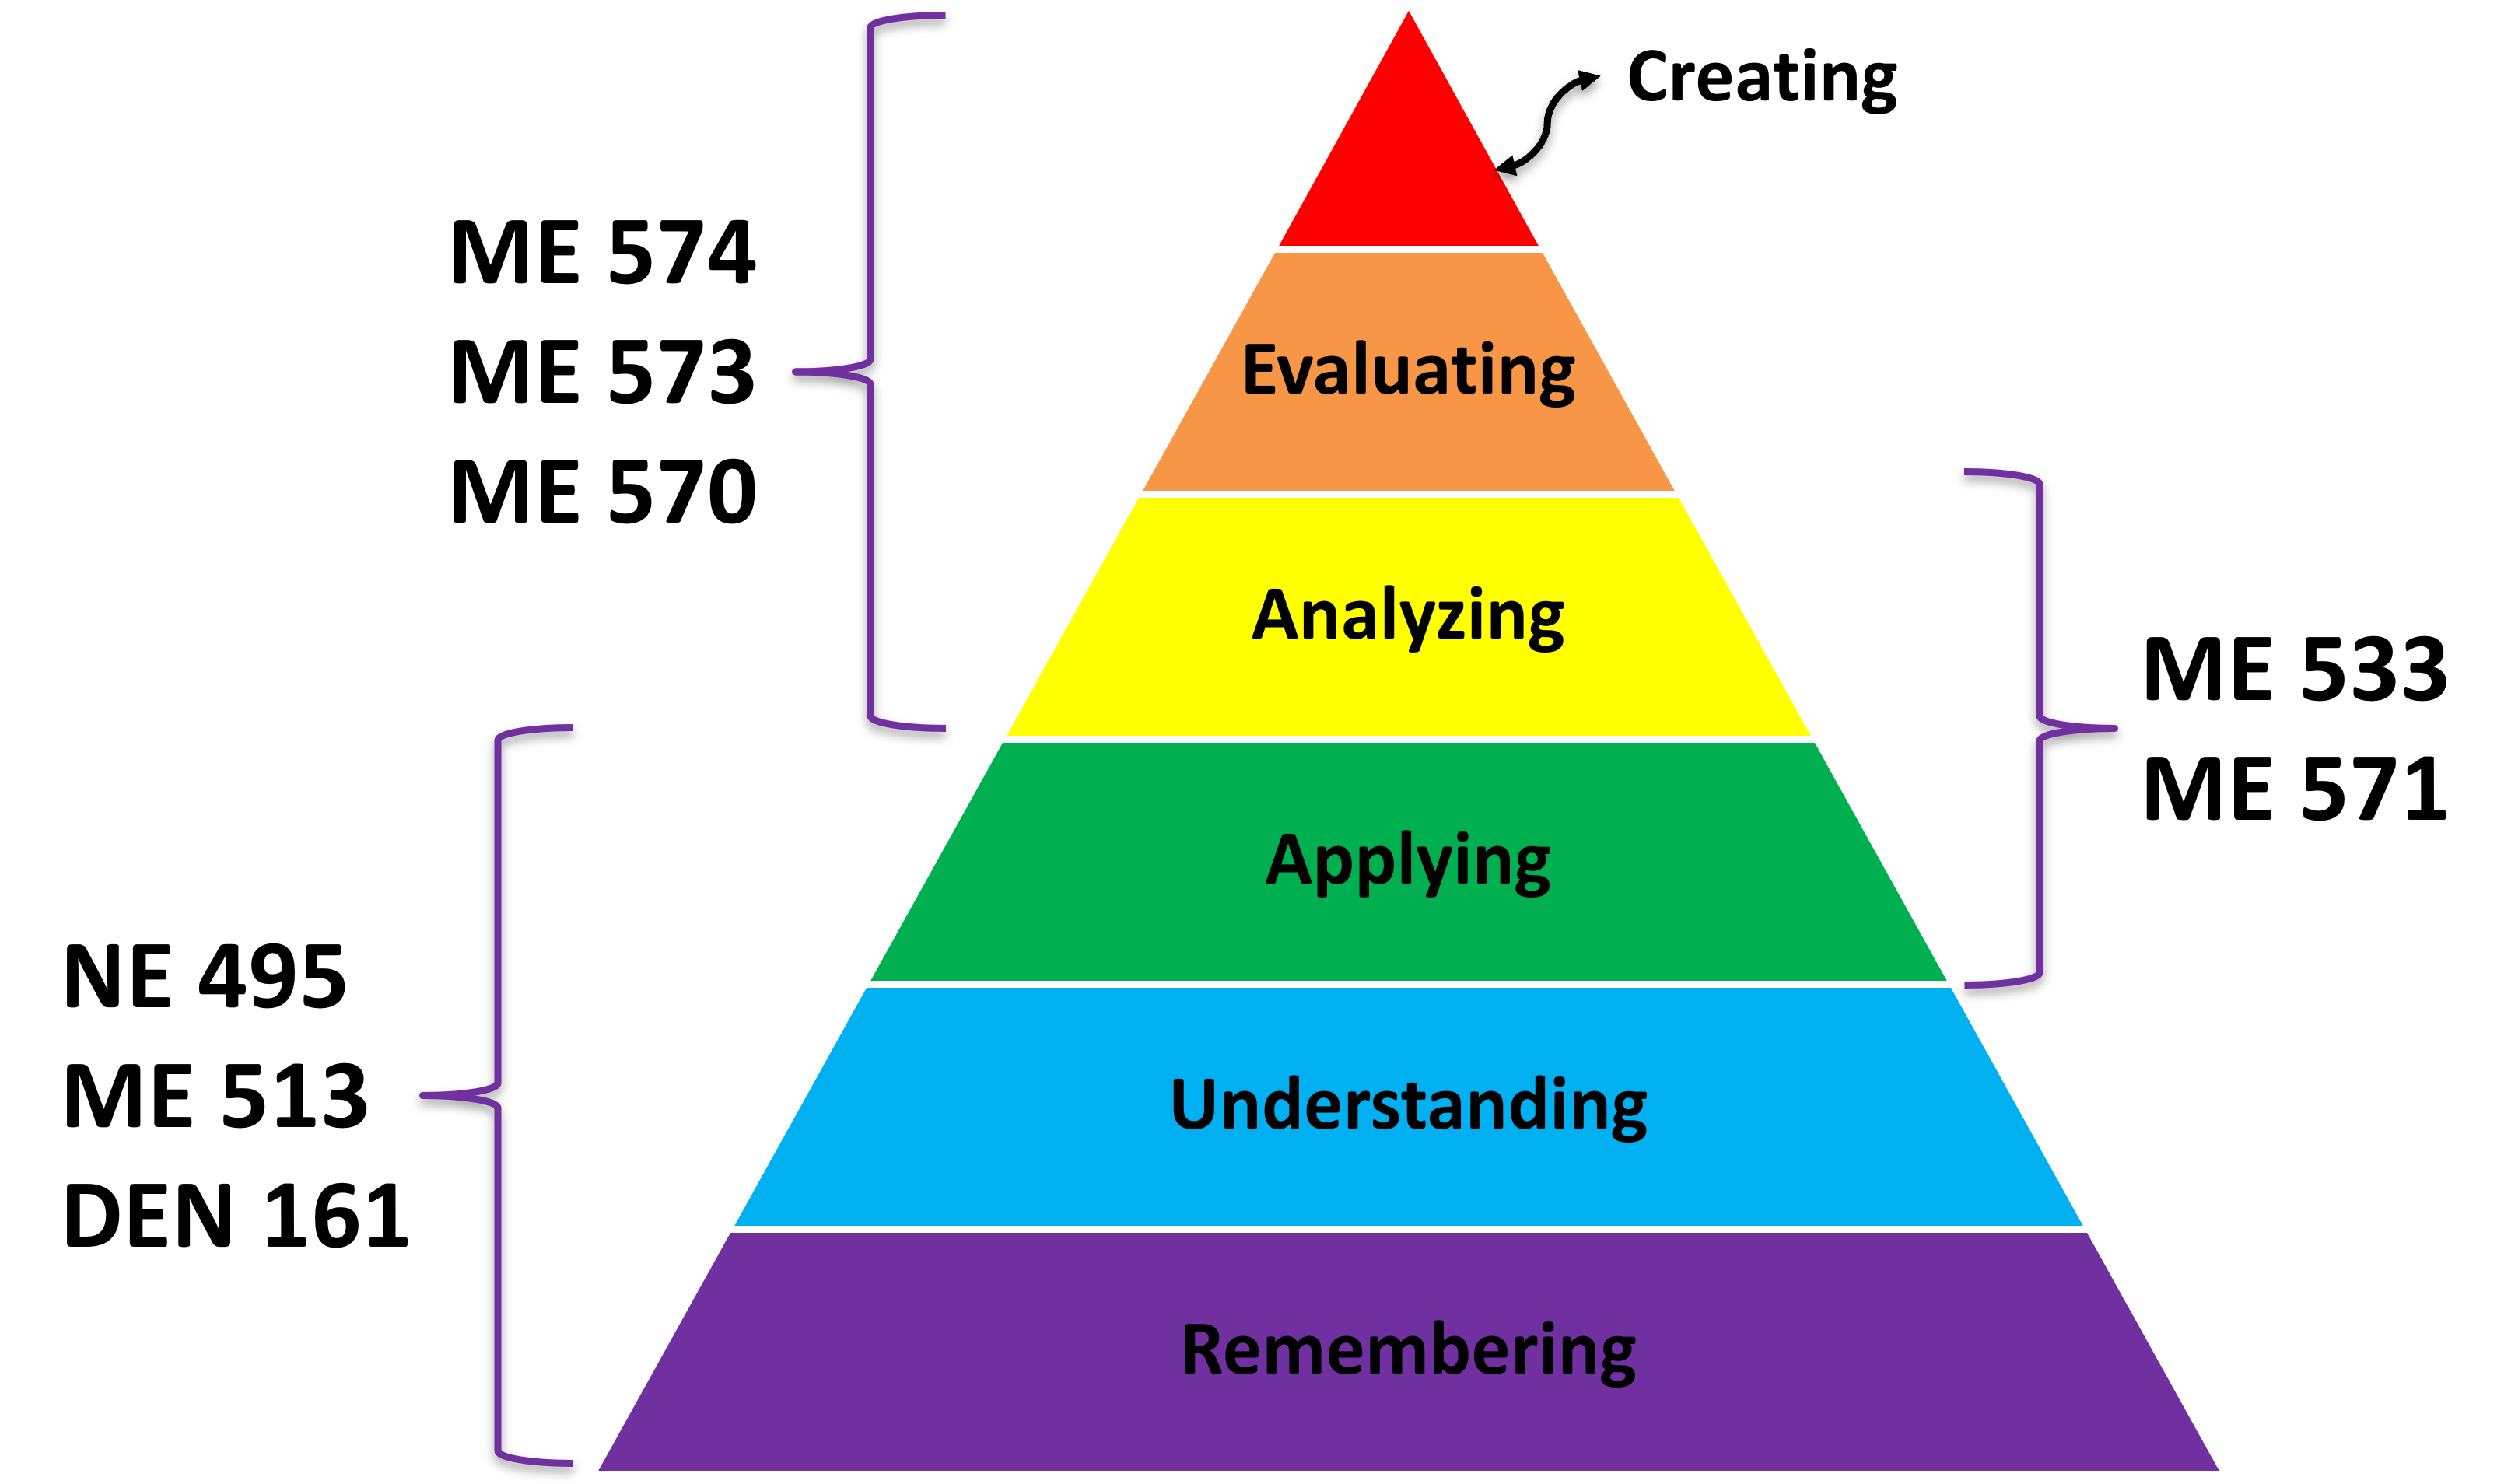
\includegraphics[width=\textwidth]{mne-curriclum-design.png}
    \caption{Progression as it relates to Bloom's Taxonomy}
    \label{revised-bloom-taxonomy}
\end{figure}

The addition of programming as a solution method in the department aligns with ABET 
Student Outcomes 1, 3, 6, and 7, which can be read in Appendix \ref{appendix:appendix_abet}.
Lastly, the use of programming, a skill-set not commonly associated with mechanical
engineers, will provide a challenge for students, as well as piquing the interest and 
motivation for students that find themselves particularly adept at coding.

Beginning with DEN 161: Engineering Problem Solving, each course chapter will contain
a brief section dedicated to recommendations for course integration based on these
principles of curriculum design. These recommendations are intended to provide insight
of the investment level needed by instructors and the students to effectively 
implement the proposed changes.